\documentclass[12pt]{article}
\usepackage[margin=1in]{geometry}
\usepackage{amsmath, amssymb}
\usepackage{graphicx}
\usepackage{float}
\usepackage{siunitx}
\usepackage{booktabs}
\usepackage{enumitem}
\usepackage{hyperref}
\usepackage{parskip}
\usepackage{cleveref}
\usepackage{tikz}
\usepackage{circuitikz}
\usepackage{xcolor}
\usepackage{listings}

\lstdefinestyle{csharp}{
  language=[Sharp]C,
  basicstyle=\ttfamily\small,
  keywordstyle=\color{blue}\bfseries,
  commentstyle=\color{teal},
  stringstyle=\color{orange},
  numbers=left,
  numberstyle=\tiny,
  stepnumber=1,
  numbersep=5pt,
  frame=single,
  breaklines=true,
  showstringspaces=false
}

\lstset{style=csharp}
\setlist[itemize]{noitemsep, topsep=0pt}
\setlist[enumerate]{label=\alph*), itemsep=0.3em}
\title{MECH 421/423 Lab 4\\Op-Amp Circuits for Noisy Environments}
\author{Gyan Edbert Zesiro \\ Student ID: 38600060}
\date{\today}
\begin{document}
\maketitle
\tableofcontents
\newpage

\section{Introduction}
This lab investigates the design of an optical distance sensor built from discrete op amp stages. Each exercise reinforces a different portion of the signal chain---from generating the optical carrier, through transimpedance conversion and filtering, to rectification, digitization, and calibration. 

\section{Methodology}
The experimental procedure was organized into three phases that progressively built up a complete optical distance sensor, from the analog front-end to digital acquisition and calibration. Each phase was completed only after verifying correct operation of the previous one.

\subsection*{Phase 1: Analog Front-End}
\begin{figure}
    \centering
    \includegraphics[width=0.8\textwidth]{images/method_circuit_1.png}
    \caption{Exercise 2 Circuit}
    \label{fig:method_circuit_1}
\end{figure}
\begin{enumerate}
    \item Configure the Analog Discovery 2 (AD2) waveform generator to drive the red LED with a \SI{5}{\volt} amplitude square wave and \SI{2.5}{\volt} DC offset. Verify visible flashing at \SI{1}{\hertz} and continuous illumination at \SI{1}{\kilo\hertz}.
    \item Mechanically mount the LED on the linear rail and align it with the photodiode on the breadboard, ensuring smooth motion and stable geometry over the full travel range.
    \item Design and assemble the photodiode transimpedance amplifier by selecting $R_2$ to convert a \SI{1}{\micro\ampere} photocurrent into a \SI{100}{\milli\volt} deviation about a bias voltage $V_1$, see \Cref{fig:method_circuit_1}.
    \item Design the bias network using $R_3$ and $R_4$ to set $V_1 \approx \SI{0.5}{\volt}$ from the \SI{5}{\volt} supply, then build and verify the bias node on the breadboard.
    \item Choose and install $R_5$ and $C_1$ to implement the first high-pass filter with a cutoff near \SI{100}{\hertz}, and confirm the expected frequency response using the AD2.
    \item Characterize the effect of ambient light by observing $V_2$ with the photodiode alternately exposed and covered, documenting the change in DC level and the small \SI{1}{\kilo\hertz} carrier component.
    \item Connect the high-pass filter output to the AC gain stage and verify that the \SI{1}{\kilo\hertz} waveform amplitude changes predictably with LED--photodiode separation over the specified distance range.
\end{enumerate}

\subsection*{Phase 2: Signal Conditioning and Rectification}
\begin{figure}
    \centering
    \includegraphics[width=0.8\textwidth]{images/method_circuit_2.png}
    \caption{Exercise 3 Circuit}
    \label{fig:method_circuit_2}
\end{figure}

Below outlines steps for Exercise 3:
\begin{enumerate}
  \item Design and construct a high-pass amplifier stage with the specified gain. 
        Choose resistors $R_7$ and $R_8$ so that the DC level at node $V_4$ is 
        $2.5~\text{V}$. Reuse $C_1$ and $R_5$ from the earlier exercises, and 
        select $R_6$ so that the overall gain is $-10$.

  \item The pair $R_6$ and $C_2$ should form a low-pass section that attenuates 
        high-frequency noise. Choose $C_2$ so that the low-pass cut-off 
        frequency is at least $16~\text{kHz}$, i.e.\ 
        $\omega_c \ge 10^{5}~\text{rad/s}$.

    \item Build the circuit shown in \Cref{fig:method_circuit_2} on your 
        breadboard.

  \item To evaluate the circuit, configure the AD2 signal generator to output a 
        $1~\text{kHz}$ sine wave with a peak amplitude of $100~\text{mV}$ and 
        apply this signal to node $V_2$.

  \item Connect the input of this filter/amplifier stage (node $V_2$) to the 
        output of the photodiode amplifier.

  \item Observe the output signal amplitude while varying the distance between 
        the LED transmitter and the photodiode receiver. The circuit should 
        produce a clearly measurable $1~\text{kHz}$ square-wave signal over 
        separation distances up to approximately $25~\text{cm}$, and the output 
        should not saturate (remain below about $5~\text{V}$) when the 
        separation is very small (less than about $3~\text{cm}$). For best 
        results, perform this distance test in a dark room with your computer 
        screen set to minimum brightness so that the photodiode primarily 
        detects light from the LED.

  \item If these conditions are not satisfied, adjust the gain of the circuit 
        as needed. This may include changing the values of $C_1$, $C_2$, $R_5$, 
        and $R_6$ until the performance meets the above criteria.
\end{enumerate}

\begin{figure}
    \centering
    \includegraphics[width=0.8\textwidth]{images/method_circuit_3.png}
    \caption{Exercise 4 Circuit}
    \label{fig:method_circuit_3}
\end{figure}
Next is exercise 4 and 5, which involves building the rectifier and low-pass filter:
\begin{enumerate}
    \item Design and build a second RC high-pass filter using $C_3$ and $R_9$ with the same cutoff frequency as the first stage to further suppress low-frequency ambient-light variations and build the Exercise 4 circuit, see \Cref{fig:method_circuit_3}.
    \item Design and construct a non-inverting rectifier stage by selecting $R_{10}$ and $R_{11}$ to achieve an overall gain of approximately $11$, ensuring that the rectified signal remains within the op-amp linear range.
    \item Design and implement a low-pass RC filter using $C_4$ and $R_{12}$ with a cutoff near \SI{1.6}{\hertz} to extract a slowly varying DC voltage proportional to the \SI{1}{\kilo\hertz} carrier amplitude.
    \item Validate the signal-conditioning chain by driving $V_5$ with a known \SI{1}{\kilo\hertz} square wave (about \SI{100}{\milli\volt} peak-to-peak) from the AD2, probing the signal after each stage (high-pass, rectifier, low-pass) and confirming the expected waveforms.
    \item Connect the output of the Phase~1 amplifier chain to this rectifier/low-pass block and adjust $R_{10}$ and $R_{11}$ if necessary so that the final output $V_{\text{out}}$ remains within the target \SIrange{0}{2.5}{\volt} range over the full LED--photodiode separation.
    \item Measure and document the steady-state output voltage versus separation distance, confirming that the circuit neither saturates at close spacing nor loses the signal at the maximum separation.
    \item Finally, connect everything together. See \Cref{fig:full_circuit} for the full circuit diagram. Then test your Vout by moving the LED along the rail and observing the output voltage change, ideally you want a noticeable change from 3cm to 25cm.
    \item Congratulations, you're done with the circuit part
\end{enumerate}

\begin{figure}
    \centering
    \includegraphics[width=0.8\textwidth]{images/method_circuit_4.png}
    \caption{Full Circuit}
    \label{fig:full_circuit}
\end{figure}

\subsection*{Phase 3: Digitization, Software, and Calibration}
\begin{enumerate}
    \item Develop firmware for the MSP430FR5739 to sample $V_{\text{out}}$ using a 10-bit ADC over a \SIrange{0}{3.3}{\volt} input range, and format each sample into two bytes (MS5B and LS5B) preceded by a synchronization byte (255).
    \item Implement a C\# application that opens the serial port, reassembles the MS5B and LS5B fields into a 10-bit digital value, and continuously displays and plots the incoming data stream.
    \item Extend the C\# user interface to log acquired data to file and provide real-time visualization suitable for tuning the sensor and verifying the dynamic behavior.
    \item Perform a calibration experiment by recording ADC output at several known separation distances across the usable range; fit an appropriate function relating ADC code to distance using numerical tools.
    \item Incorporate the calibration function into the C\# program so that it converts each ADC reading into a distance estimate, displays both raw and converted values, and flags out-of-range conditions.
    \item Quantify the sensor resolution by logging the converted distance at a fixed nominal position for an extended period, computing the standard deviation of the measured distance, and repeating near the ends of the operating range to compare noise performance.
\end{enumerate}

\section{Phase 1: Analog Front-End}
\subsection{Exercise 1: Optical Transmitter}
\subsubsection{Question 1: Assemble and Power the LED}
I've built the distance sensor with the guide rail. This will be crucial later to get accurate and precise distance measurement.

\subsubsection{Question 2: Verify 1~Hz Modulation}
With the generator at 1~Hz the LED visibly flashed,

\subsubsection{Question 3: Verify 1~kHz Modulation}
if you choose 1~kHz waveform, the LED appear continuously on, indicating that the chosen frequency exceeds the flicker fusion threshold and is suitable as the optical carrier for later exercises.

\subsection{Exercise 2: Photodiode Amplifier and High-Pass Filter}
\subsubsection{Question 1: Choose \texorpdfstring{$R_2$}{R2}}
Using the constraint $\Delta V_2 = \SI{100}{\milli\volt}$ for a \SI{1}{\micro\ampere} photocurrent,
\begin{align*}
    R_2 &= \frac{\Delta V_2}{I_d}=\frac{0.1}{1\times 10^{-6}} = \SI{100}{\kilo\ohm}.
\end{align*}

\subsubsection{Question 2: Choose \texorpdfstring{$R_3$}{R3} and \texorpdfstring{$R_4$}{R4}}
Bias $V_1$ at \SI{0.5}{\volt} using a divider referenced to \SI{5}{\volt}:
\begin{align*}
    V_1 &= \frac{R_4}{R_3+R_4} V_{\text{ref}} = 0.5.
\end{align*}
Selecting $R_3 = \SI{200}{\kilo\ohm}$ and $R_4 = \SI{22}{\kilo\ohm}$ yields
\begin{align*}
    V_1 &= \frac{22}{200+22}\times 5 \approx \SI{0.495}{\volt},
\end{align*}
which is sufficiently close to the target bias.

Then you just have to build the circuit, see \Cref{fig:2_2_result} for the breadboard circuit diagram.

\begin{figure}
    \centering
    \includegraphics[width=0.8\textwidth]{images/2_3-circuit.jpg}
    \caption{Breadboard circuit diagram for Exercise 2}
    \label{fig:2_2_result}
\end{figure}

\subsubsection{Question 3: Choose \texorpdfstring{$R_5$}{R5} and \texorpdfstring{$C_1$}{C1}}
For the filter design, the transfer function amplitude is equal to $\frac{1}{\sqrt{2}}$ at the cutoff frequency:
\begin{align*}
\left| \frac{R}{R + \dfrac{1}{\omega C}} \right|
  &= \frac{1}{\sqrt{2}} \\[6pt]
\left| \frac{\omega R C j}{\omega R C j + 1} \right|
  &= \frac{1}{\sqrt{2}} \\[6pt]
\frac{(\omega R C)^2}{1 + (\omega R C)^2}
  &= \frac{1}{2} \\[6pt]
2(\omega R C)^2 &= 1 + (\omega R C)^2 \\[6pt]
(\omega R C)^2 &= 1 \\[6pt]
\omega R C &= 1 \\[6pt]
RC &= \frac{1}{\omega}
      = \frac{1}{2\pi \cdot 100} \\[6pt]
RC &\approx \boxed{1.59155 \times 10^{-3}\ \text{s}}
\end{align*}

R$_5 = 1.6~\text{k}\Omega$, \quad C$_1 = 1~\mu\text{F}$ are good enough

\subsubsection{Question 4: Demonstrate Ambient-Light Impact}
\begin{figure}[H]
    \centering
    \includegraphics[width=0.8\textwidth]{images/2_4-open.png}
    \caption{Waveform when photodiode is exposed to ambient light.}
    \label{fig:ambient_light}
\end{figure}

\begin{figure}[H]
    \centering
    \includegraphics[width=0.8\textwidth]{images/2_4-close.png}
    \caption{Waveform when photodiode is covered.}
    \label{fig:covered_photodiode}
\end{figure}
\Cref{fig:ambient_light} shows $V_2$ with the photodiode exposed to room light while \Cref{fig:covered_photodiode} shows the effect of covering it. As you can see, covering the photodiode reduces the DC offset, which is what we expected.


\subsubsection{Question 5: Detect the \SI{1}{\kilo\hertz} Carrier at \texorpdfstring{$V_2$}{V2}}
First, setup the LED by using the AD2 waveform generator, connect the positive of the waveform to the anode of the LED and the negative to the cathode of the LED. Set the waveform generator to output a \SI{2.5}{\volt} amplitude square wave with a \SI{2.5}{\volt} DC offset at \SI{1}{\kilo\hertz}. \Cref{fig:wavegen_setup} shows the setup inside the WaveForm software.
\begin{figure}[H]
    \centering
    \includegraphics[width=0.8\textwidth]{images/2_5-wavegen_setup.png}
    \caption{Waveform generator setup for LED modulation}
    \label{fig:wavegen_setup}
\end{figure}
After setting up the LED, bring the LED close to the photodiode, and observe the voltage using the AD2 oscilloscope at $V_2$.
\begin{figure}[H]
    \centering
    \includegraphics[width=0.8\textwidth]{images/2_5-result.png}
    \caption{Waveform at $V_2$ with LED close to photodiode.}
    \label{fig:2_5_result}
\end{figure}
The resulting waveform is shown in \Cref{fig:2_5_result}. Notice that this is a 1khz square wave signal (just count that there is 5 cycles in 5ms)

This is what we should expect, here is the math for our result:

Let the photodiode current be written as the sum of a DC component due to
ambient light and an AC component due to the modulated LED,
\[
i_{\text{ph}}(t) = I_{\text{amb}} + \Delta I\,q(t),
\]
where \(q(t)\) is a unit-amplitude, zero-mean square wave of frequency
\(f_0 = 1~\text{kHz}\) (i.e.\ \(q(t) = \pm 1\) with 50\% duty cycle), and
\(\Delta I\) is the amplitude of the photocurrent variation when the LED
is driven.

The op-amp is configured as a transimpedance amplifier referenced to
\(V_1\).  Because of the virtual short between the inputs, the inverting
node is held at
\[
V_- \approx V_+ = V_1.
\]
Applying KCL at the inverting node gives
\[
\frac{V_2(t) - V_1}{R_2} = - i_{\text{ph}}(t),
\]
so the output voltage of the transimpedance stage is
\[
V_2(t) = V_1 - R_2\,i_{\text{ph}}(t)
       = \bigl(V_1 - R_2 I_{\text{amb}}\bigr)
         - R_2 \Delta I\, q(t).
\]
Thus \(V_2(t)\) consists of a DC offset
\[
V_{2,\text{DC}} = V_1 - R_2 I_{\text{amb}}
\]
plus a \(1~\text{kHz}\) square-wave component of peak amplitude
\[
V_{2,\text{AC}}(t) = - R_2 \Delta I\, q(t),
\]
so the peak-to-peak value of the \(1~\text{kHz}\) component at \(V_2\)
is
\[
V_{2,\text{pp}} = 2 R_2 \Delta I.
\]
As the LED–photodiode distance changes, \(\Delta I\) changes, and the
square-wave amplitude at \(V_2\) scales linearly with the photocurrent
variation.


\subsubsection{Question 6: Observe the High-Pass Output}
\begin{figure}
    \centering
    \includegraphics[width=0.8\textwidth]{images/2_6-result.png}
    \caption{Waveform at $V_3$ with LED close to photodiode.}
    \label{fig:2_6_result}
\end{figure}
The result at $V_3$ is shown in \Cref{fig:2_6_result}. 

The node \(V_2\) is now applied to the high-pass filter formed by \(C_1\)
and \(R_5\).  Taking \(V_2(t)\) as the input and \(V_3(t)\) as the
output, the transfer function of this first-order high-pass filter is
\[
H(s) = \frac{V_3(s)}{V_2(s)}
     = \frac{s R_5 C_1}{1 + s R_5 C_1}.
\]
For a sinusoidal component of angular frequency \(\omega\),
\[
H(j\omega) = \frac{j\omega R_5 C_1}{1 + j\omega R_5 C_1},
\]
and its magnitude is
\[
\bigl|H(j\omega)\bigr|
= \frac{\omega R_5 C_1}{\sqrt{1 + (\omega R_5 C_1)^2}}.
\]

The cut-off angular frequency is chosen as
\[
\omega_c = \frac{1}{R_5 C_1} \approx 500~\text{rad/s}
\quad (\text{about }100~\text{Hz}),
\]
so at the LED modulation frequency \(f_0 = 1~\text{kHz}\),
\(\omega_0 = 2\pi f_0\), we have
\[
\omega_0 R_5 C_1 = \frac{\omega_0}{\omega_c}
= \frac{2\pi \cdot 1000}{500} \approx 12.6,
\]
and therefore
\[
\bigl|H(j\omega_0)\bigr|
= \frac{12.6}{\sqrt{1 + 12.6^2}}
\approx 0.997 \approx 1.
\]

The DC term \(V_{2,\text{DC}}\) is completely blocked by the high-pass
filter (its gain at \(\omega = 0\) is zero), while the \(1~\text{kHz}\)
square-wave component passes essentially unchanged in amplitude.
Therefore the output at \(V_3\) is approximately
\[
V_3(t) \approx \bigl|H(j\omega_0)\bigr|\,
             V_{2,\text{AC}}(t)
         \approx - R_2 \Delta I\, q(t),
\]
with a peak-to-peak value
\[
V_{3,\text{pp}} \approx \bigl|H(j\omega_0)\bigr|\,V_{2,\text{pp}}
                 \approx V_{2,\text{pp}}
                 = 2 R_2 \Delta I.
\]

Hence, at \(V_3\) we observe a square wave at \(1~\text{kHz}\) whose
peak-to-peak amplitude is essentially the same as the AC component of
\(V_2\), but now centered around \(0~\text{V}\) rather than around the
bias voltage \(V_1\). As the distance between the LED and photodiode is
changed, \(\Delta I\) changes, and the peak-to-peak amplitude at \(V_3\)
varies proportionally, which is what I found experimentally (and hopefully you too).

\subsubsection{Question 7: Hardware Arrangement}
Follow the instruction and you'll end up with the setup shown in the lab manual. Note that this is very crucial for later experiments.
Because you need to align the photodiode and LED properly, make sure that the LED is facing the photodiode directly. I experienced a lot
of issues because of misalignment, particularly I couldn't get the full range of distance measurement because the photodiode couldn't "see" the LED properly. So future mechatronics student, please pay attention to this. If you're not convinced, I have derivation once we build the full circuit.

\subsection{Exercise 3: High-Pass Filter and AC Amplifier}
\subsubsection{Question 1: Bias Network}
% --- 1) Choice of R8 and R7 ---
\begin{align}
\frac{R_8}{R_8 + R_7} &= \frac{1}{2} \\[4pt]
2 R_8 &= R_8 + R_7 \\[4pt]
R_8 &= R_7
\end{align}

We can choose, for example,
\begin{align}
R_8 = R_7 &= \boxed{10~\text{k}\Omega}.
\end{align}

% --- 2) Equivalent impedances Z1 and Z2 ---
The input and feedback impedances of the op-amp stage are
\begin{align}
Z_1 &= R_5 + \frac{1}{s C_1}
     = \frac{1 + s R_5 C_1}{s C_1}, \\[6pt]
Z_2 &= R_6 \parallel \frac{1}{s C_2}
     = \frac{R_6}{R_6 + \dfrac{1}{s C_2}}
     = \frac{R_6}{1 + s R_6 C_2}.
\end{align}

% --- 3) Output expression V0 in terms of V2 and V4 ---
For the non-inverting configuration, with \(V_4\) at the non-inverting input
and \(V_2\) feeding the inverting node through \(Z_1\), the output is
\begin{align}
V_0 &= V_4\!\left(1 + \frac{Z_2}{Z_1}\right)
      - V_2 \left(\frac{Z_2}{Z_1}\right) \\[4pt]
    &= V_4 + \frac{Z_2}{Z_1}\left(V_4 - V_2\right).
\end{align}

% --- 4) Gain condition |Z2/Z1| = 10 ---
We want the magnitude of the transfer ratio to be about 10:
\begin{align}
\left|\frac{Z_2}{Z_1}\right| &\approx 10.
\end{align}

Compute the ratio:
\begin{align}
\frac{Z_2}{Z_1}
  &= \frac{\dfrac{R_6}{1 + s R_6 C_2}}
          {R_5 + \dfrac{1}{s C_1}} \\[6pt]
  &= \frac{R_6}{1 + s R_6 C_2}
     \cdot \frac{s C_1}{1 + s R_5 C_1} \\[6pt]
  &= \frac{R_6}{R_5} \;
     \frac{s R_5 C_1}{1 + s R_5 C_1}
     \cdot \frac{1}{1 + s R_6 C_2}.
\end{align}

In the midband of interest (where the frequency-dependent factors are near
unity), the dominant term is \(R_6/R_5\), so we choose
\begin{align}
\frac{R_6}{R_5} &\approx \boxed{10}.
\end{align}

Then we can choose our resistor, which in this case I choose to be:
\begin{align}
R_5 &= \boxed{1.6~\text{k}\Omega}, \\
R_6 &= \boxed{16~\text{k}\Omega}.
\end{align}

\subsubsection{Question 2: Choose \texorpdfstring{$C_2$}{C2}}
The feedback network $R_6$--$C_2$ implements a first–order low-pass term of the form  
\[
H_{\text{LP}}(j\omega) = \frac{1}{1 + j\omega R_6 C_2}.
\]
The magnitude is
\begin{align*}
\left| H_{\text{LP}}(j\omega) \right|
  &= \left| \frac{1}{1 + j\omega R_6 C_2} \right|
   = \frac{1}{\sqrt{1 + (\omega R_6 C_2)^2}}.
\end{align*}
The $-3\,\mathrm{dB}$ cut-off occurs when $\lvert H_{\text{LP}}(j\omega_c)\rvert = 1/\sqrt{2}$:
\begin{align*}
\frac{1}{\sqrt{1 + (\omega_c R_6 C_2)^2}} &= \frac{1}{\sqrt{2}} \\
1 + (\omega_c R_6 C_2)^2 &= 2 \\
(\omega_c R_6 C_2)^2 &= 1 \\
\omega_c R_6 C_2 &= 1 \\
C_2 &= \frac{1}{\omega_c R_6}.
\end{align*}

With $R_6 = \SI{16}{k\ohm}$ and the desired cut-off
$f_c = \SI{16}{kHz}$ (so $\omega_c = 2\pi f_c \approx 1.01\times10^5\ \mathrm{rad/s}$),
\begin{align*}
C_2 
  &= \frac{1}{(2\pi f_c) R_6} \\
  &= \frac{1}{(2\pi)(16\times10^3)(16\times10^3)} \\
  &\approx 6.22\times 10^{-10}\ \mathrm{F}
   = 0.622\ \mathrm{nF}
   \approx 620\ \mathrm{pF}.
\end{align*}
Thus the ideal design value is
\[
\boxed{C_2 \approx \SI{0.622}{nF} \approx \SI{620}{pF}}.
\]

In the lab, the largest available capacitor not exceeding this value was
$C_2 = \SI{100}{pF}$. Using this component shifts the pole to a higher
frequency:
\begin{align*}
\omega_{c,\text{actual}} 
  &= \frac{1}{R_6 C_2}
   = \frac{1}{(16\times10^3)(100\times10^{-12})}
   = 6.25\times10^5\ \mathrm{rad/s}, \\
f_{c,\text{actual}}
  &= \frac{\omega_{c,\text{actual}}}{2\pi}
   \approx 9.95\times10^4\ \mathrm{Hz}
   \approx \SI{100}{kHz}.
\end{align*}
So the implemented filter still satisfies the specification
($\omega_c \ge 10^5\ \mathrm{rad/s}$) while providing even stronger
attenuation of higher-frequency interference:
\[
\boxed{C_2 = \SI{100}{pF},\quad f_{c,\text{actual}} \approx \SI{100}{kHz}.}
\]

so what is this circuit doing? below are the derivation to see what is happening.


For small AC signals, the bias node $V_4 \approx 2.5~\text{V}$ is a DC
level, so its AC value is effectively zero.  
Thus, the non-inverting input is at AC ground and the op-amp works as an
\emph{inverting} amplifier with:

\[
V_2 \xrightarrow{\;C_1,\,R_5\;} \text{inverting node}, \qquad
V_5 \xrightarrow{\;R_6 \parallel C_2\;} \text{feedback}.
\]

Define
\begin{align*}
Z_1 &= R_5 + \frac{1}{s C_1} &&\text{(series input impedance)},\\[4pt]
Z_2 &= R_6 \parallel \frac{1}{s C_2}
     = \frac{R_6}{1 + s R_6 C_2} &&\text{(feedback impedance)}.
\end{align*}

With the inverting-node voltage $\approx 0$ (ideal op-amp),
Kirchhoff's current law gives
\begin{align*}
\frac{V_2(s) - 0}{Z_1} + \frac{V_5(s) - 0}{Z_2} &= 0,\\[4pt]
\Rightarrow\quad
\boxed{\displaystyle
\frac{V_5(s)}{V_2(s)} = -\,\frac{Z_2}{Z_1}
}.
\end{align*}

Substitute $Z_1$ and $Z_2$:
\begin{align*}
\frac{V_5(s)}{V_2(s)}
&= -\,\frac{\dfrac{R_6}{1 + s R_6 C_2}}
          {R_5 + \dfrac{1}{s C_1}} \\[6pt]
&= -\,\frac{R_6}{1 + s R_6 C_2}
      \cdot \frac{s C_1}{1 + s R_5 C_1} \\[6pt]
&= \boxed{\frac{R_6}{R_5}
\left(\frac{s R_5 C_1}{1 + s R_5 C_1}\right)
\left(\frac{1}{1 + s R_6 C_2}\right)
}
\end{align*}

This shows:
\begin{itemize}
  \item $C_1$ and $R_5$ form a \textbf{high-pass} with cutoff
        $\omega_{\mathrm{HP}} = \dfrac{1}{R_5 C_1}$.
  \item $R_6$ and $C_2$ form a \textbf{low-pass} with cutoff
        $\omega_{\mathrm{LP}} = \dfrac{1}{R_6 C_2}$.
  \item In between these two cutoffs,
        the gain tends to the constant
        \(\dfrac{R_6}{R_5}\) (inverting amplifier).
\end{itemize}



Go ahead and built the circuit, see \Cref{fig:ex_3_circuit} for my breadboard circuit implementation.

\begin{figure}
    \centering
    \includegraphics[width=0.8\textwidth]{images/3_3-circuit.jpg}
    \caption{Breadboard circuit diagram for Exercise 3}
    \label{fig:ex_3_circuit}
\end{figure}

\subsubsection{Question 3: Verification}
Configure your waveform generator to 100 mV amplitude 1 kHz sine wave using the AD2 signal generator and 
connect it to V2. Then use your oscilloscope to measure the output at V5. You should see a sine wave at V5. Measure the amplitude of the output sine wave at V5. Vary the frequency to see it's effect on the output amplitude.
Here are my result for 1khz, 100khz, and 1mhz:
\begin{figure}[H]
    \centering
    \includegraphics[width=0.8\textwidth]{images/3_3-1khz.png}
    \caption{Waveform at $V_5$ with 1 kHz input.}
    \label{fig:4_3_1khz}
\end{figure}
\begin{figure}[H]
    \centering
    \includegraphics[width=0.8\textwidth]{images/3_3-100khz.png}
    \caption{Waveform at $V_5$ with 100 kHz input.}
    \label{fig:4_3_100khz}
\end{figure}
\begin{figure}[H]
    \centering
    \includegraphics[width=0.8\textwidth]{images/3_3-1000khz.png}
    \caption{Waveform at $V_5$ with 1 MHz input.}
    \label{fig:4_3_1mhz}
\end{figure}
\subsection*{Frequency response and output amplitudes}

Let the input at $V_2$ be a sine wave
\[
v_2(t) = \hat V_2 \sin(\omega t),
\qquad \hat V_2 = 0.1~\text{V} \; (100~\text{mV}).
\]
The complex gain at frequency $\omega$ is
\[
A(j\omega) = \frac{V_5(j\omega)}{V_2(j\omega)}
           = \frac{R_6}{R_5}
\left(\frac{s R_5 C_1}{1 + s R_5 C_1}\right)
\left(\frac{1}{1 + s R_6 C_2}\right).
\]
The output amplitude is
\[
\hat V_5 = \left|A(j\omega)\right|\hat V_2.
\]

If we go through the calculations, these are the amplitude modulations at
different frequencies for our circuit (assuming R6/R5 = 10):
\[
\boxed{
\hat V_5 \approx
\begin{cases}
9.99999~\text{V}, & f = 1~\text{kHz},\\[2pt]
5.3~\text{V}, & f = 100~\text{kHz},\\[2pt]
0.62~\text{V}, & f = 1~\text{MHz}.
\end{cases}
}
\]

My result is similar to our calculation
(\(1.044~\text{V}\), \(0.514~\text{V}\), \(64.2~\text{mV}\))
are of the same order, so everything seems to check out. I believe
this is reasonable given tolerances in the actual resistor/capacitor
values, and can also be caused by the
bandwidth and slew-rate limits of the real op-amp.
\subsection{Exercise 4: High-Pass Filter, Rectifier, and Low-Pass Filter}
\subsubsection{Question 1: Duplicate High-Pass}
This stage reused the Exercise~2 sizing so $R_9 = \SI{1.6}{\kilo\ohm}$ and $C_3 = \SI{1}{\micro\farad}$, keeping the \SI{100}{\hertz} cutoff.

\subsubsection{Question 2: Rectifier Gain}

\begin{align*}
V_7 &= V_6\!\left(1 + \frac{R_{11}}{R_{10}}\right), \\
\frac{R_{11}}{R_{10}} &= 10
      \quad\Rightarrow\quad
      \boxed{R_{10} = 1~\text{k}\Omega,\; R_{11} = 10~\text{k}\Omega\ \text{works}.}
\end{align*}


\subsubsection{Question 3: Low-Pass Filter}
\begin{align*}
V_8 &= \frac{\dfrac{1}{sC_4}}{\dfrac{1}{sC_4} + R_{12}}\,V_7 \\
    &= \frac{1}{1 + R_{12}sC_4}\,V_7
\end{align*}

For the \(-3\:\text{dB}\) point we set \(s = j\omega\) and
\begin{align*}
\left|\frac{1}{1 + j\omega R_{12}C_4}\right|
  &= \frac{1}{\sqrt{2}} \\
1 + (\omega R_{12}C_4)^2 &= 2 \\
\omega R_{12}C_4 &= 1 \\
R_{12}C_4 &= \frac{1}{\omega}
          = \frac{1}{1.6\cdot 2\pi}
          \approx 9.95\times 10^{-2}.
\end{align*}

\[
\boxed{C_4 = 100~\text{nF}},\qquad
\boxed{R_{12} = 1~\text{M}\Omega}
\]


\subsubsection{Question 4: Response Checks}
The next step is to check if your circuit works for Exericse 3 number 4, 5, 6. This is the perfect time for you to test if your circuit
has the full 2.5V range. If the range is bad, please first try aligning your photodiode, because that might be the number one cause of this issue.
Below are my results for V6, V7, and V8:
\begin{figure}[H]
    \centering
    \includegraphics[width=0.8\textwidth]{images/4_4-v6.png}
    \caption{Waveform at $V_6$.}
    \label{fig:4_4_v6}
\end{figure}
\begin{figure}[H]
    \centering
    \includegraphics[width=0.8\textwidth]{images/4_4-v7.png}
    \caption{Waveform at $V_7$.}
    \label{fig:4_4_v7}
\end{figure}
\begin{figure}[H]
    \centering
    \includegraphics[width=0.8\textwidth]{images/4_4-v8.png}
    \caption{Waveform at $V_8$.}
    \label{fig:4_4_v8}
\end{figure}

Notice that V8 is a constant line, which is great for our data acquisition system. This is the outline on the output of V8:
The last stage is a simple RC low–pass with input \(V_7\) and output \(V_8\):
a resistor \(R_{12}\) in series, a capacitor \(C_4\) to ground at the output node.
Its transfer function is
\begin{align*}
H(s) &= \frac{V_8(s)}{V_7(s)}
     = \frac{1}{1 + s R_{12} C_4},
\end{align*}
so in the frequency domain
\begin{align*}
H(j\omega) &= \frac{1}{1 + j \omega R_{12} C_4}, \\
\bigl|H(j\omega)\bigr|
  &= \frac{1}{\sqrt{1 + (\omega R_{12} C_4)^2}}.
\end{align*}

The cut–off frequency is
\begin{align*}
\omega_c &= \frac{1}{R_{12} C_4} = 10~\text{rad/s}
           \quad\Rightarrow\quad
f_c = \frac{\omega_c}{2\pi} \approx 1.6~\text{Hz},
\end{align*}
so we can write
\begin{align*}
\bigl|H(j\omega)\bigr|
= \frac{1}{\sqrt{1 + (\omega/\omega_c)^2}}
= \boxed{\displaystyle
\frac{1}{\sqrt{1 + (\omega/10)^2}}
}.
\end{align*}

\subsection*{Effect on the rectified 1 kHz waveform}

Let the rectifier output \(V_7(t)\) be decomposed into a DC component
plus an AC component with fundamental frequency \(f_0 = 1~\text{kHz}\):
\begin{align*}
V_7(t) &= V_{\text{DC}} + v_{\text{AC}}(t), \\
v_{\text{AC}}(t) &= \sum_{n=1}^{\infty}
A_n \cos\!\bigl(n \omega_0 t + \phi_n\bigr),
\qquad \omega_0 = 2\pi f_0 .
\end{align*}
(For a rectified square wave this is a Fourier series with harmonics of
\(1~\text{kHz}\).)

The DC term is at \(\omega = 0\), so
\begin{align*}
\bigl|H(j0)\bigr| &= 1,
\end{align*}
i.e.\ the DC level passes unchanged.

For the AC harmonics, each component at frequency \(n\omega_0\)
is multiplied by \(\bigl|H(jn\omega_0)\bigr|\):
\begin{align*}
v_{\text{AC,out}}(t)
&= \sum_{n=1}^{\infty}
A_n \bigl|H(j n \omega_0)\bigr|
    \cos\!\bigl(n \omega_0 t + \phi_n + \angle H(jn\omega_0)\bigr).
\end{align*}

Now compute the attenuation for the fundamental at \(1~\text{kHz}\):
\begin{align*}
\omega_0 &= 2\pi \times 10^3 \approx 6.283\times 10^3~\text{rad/s},\\[4pt]
\frac{\omega_0}{\omega_c} &= \frac{6.283\times 10^3}{10} \approx 628.3,\\[4pt]
\bigl|H(j\omega_0)\bigr|
&= \frac{1}{\sqrt{1 + (628.3)^2}}
 \approx \boxed{1.6\times 10^{-3}}.
\end{align*}
So the 1 kHz ripple at the output is only about \(0.16\%\) of the ripple
at \(V_7\).  
Higher harmonics (\(n\ge2\)) are at even larger frequencies
\(n\omega_0\), so
\begin{align*}
\bigl|H(j n\omega_0)\bigr|
&= \frac{1}{\sqrt{1 + (n\omega_0/\omega_c)^2}}
\ll 1.6\times 10^{-3}
\qquad (n \ge 2),
\end{align*}
and are suppressed even more strongly.

Therefore the output is
\begin{align*}
V_8(t)
&= V_{\text{DC}}\cdot 1 \;+\; v_{\text{AC,out}}(t)\\
&\approx V_{\text{DC}} \;+\; \text{(very small ripple)}.
\end{align*}

On the oscilloscope, this tiny residual ripple is far below the vertical
scale and you see essentially only the DC term:
\begin{align*}
\boxed{V_8(t) \approx V_{\text{DC}} = \text{constant line}.}
\end{align*}

Intuitively, the time constant of the low–pass filter is
\(\tau = R_{12}C_4 = 1/\omega_c = 0.1~\text{s}\), whereas the period of
the 1 kHz waveform is \(T = 1~\text{ms} \ll \tau\).  
The capacitor voltage cannot change much within one period of the
waveform, so the filter effectively averages the rectified signal and
outputs an almost constant DC value.

\subsection{Exercise 5: Assemble Complete Circuit}
Below are the complete circuit diagram for Exercise 4, and also for Exercise 5:
\begin{figure}
    \centering
    \includegraphics[width=0.8\textwidth]{images/4_3-circuit.jpg}
    \caption{Breadboard circuit diagram for Exercise 4 and Exercise 5}
    \label{fig:ex_4_circuit}
\end{figure}
\subsubsection{Question 1: Integrate Stages}
Finally, we are done with our circuit, the next step is to wire together the transimpedance amplifier (Exercise~2), AC amplifier (Exercise~3), and rectifier/low-pass chain (Exercise~4) to form the complete sensor. After this check all the connections again to make sure everything is correct. Once you are sure everything is correct, power up the circuit and test if it works as expected. 

\subsubsection{Question 2: Constrain Output Range}
If everything is correct, you should be able to see the output voltage $V_{\text{out}}$ vary between 0~V and 2.5~V as you sweep the LED along the rail. It's okay if you don't get the full range, as long as it's close to 2.5V that's good enough. 
After following the advice of our TA to get good alignnment, I managed to get a full voltage of 2.3V when the LED is close, which is good enough.

\section{Phase 3: Data Acquisition and Calibration}

\subsection{The Importance of Alignment with Photodiode and LED}
I was struggling to get the full range of 2.5V output for a while, but thanks to our TA, he informed me that the alignment between the photodiode and LED is very crucial. To convince you, here is a simple math behind it:

For clarity, \Cref{fig:alignment_geometry} shows the simplified geometry
used in the small-angle discussion. This figure will be the basis for our derivation.
\begin{figure}[H]
    \centering
    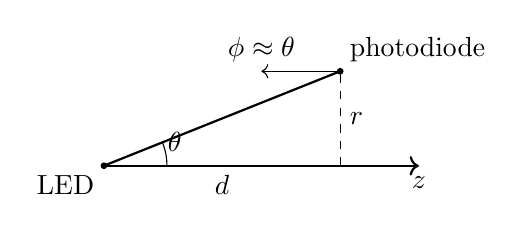
\begin{tikzpicture}[scale=1.0]
        % LED at origin
        \filldraw[black] (0,0) circle (1pt) node[below left] {LED};
        \draw[->,thick] (0,0) -- (4,0) node[below] {$z$};

        % Photodiode position
        \coordinate (PD) at (3,1.2);
        \filldraw[black] (PD) circle (1pt);
        \draw (PD) node[above right] {photodiode};

        % Distance components
        \draw[dashed] (0,0) -- (3,0) node[midway, below] {$d$};
        \draw[dashed] (3,0) -- (PD) node[midway, right] {$r$};
        \draw[thick] (0,0) -- (PD);

        % Angle theta at LED
        \draw (0.8,0) arc[start angle=0,end angle=21.8,radius=0.8];
        \node at (0.9,0.3) {$\theta$};

        % Photodiode normal (assumed perpendicular to LED axis)
        \draw[->] (PD) -- ++(-1,0) node[above]{$\phi \approx \theta$};
    \end{tikzpicture}
    \caption{Geometry for lateral misalignment $r$ between LED and photodiode.}
    \label{fig:alignment_geometry}
\end{figure}
\subsubsection*{Assumptions for the ``LED close'' case}

Here I only care about what happens when the LED is \emph{already close} to
the photodiode (say $d \approx \SI{3}{\centi\meter}$) and we introduce a
small angular misalignment.  The assumptions are
\begin{itemize}
    \item The LED is a Lambertian source of order $m$, so the radiant
          intensity versus angle $\theta$ from its optical axis is
          \[
              I(\theta) = I_0 \cos^{m} \theta.
          \]
          For a typical narrow LED with half-power angle
          $\theta_{1/2} \approx 15^\circ$,
          \[
              m = -\frac{\ln 2}{\ln(\cos\theta_{1/2})} \approx 20.
          \]
    \item The photodiode follows a cosine law with respect to its surface
          normal, so the received flux has an extra factor $\cos\theta$ when
          we tilt away from perfect alignment.
    \item At \SI{1}{\kilo\hertz} the electronic chain is linear with an
          overall gain from photocurrent swing $\Delta I$ to final DC output
          $V_{\text{out}}$:
          \[
              V_{\text{out}} = G_{\text{sys}}\,\Delta I,
          \]
          where
          \[
              G_{\text{sys}}
              \approx R_2 \times 10 \times 11
              = (100\,\text{k}\Omega)\times 10\times 11
              \approx 1.1\times 10^{7}\ \frac{\text{V}}{\text{A}}.
          \]
          Here $R_2$ is the transimpedance gain, $10$ is the midband gain of
          the AC amplifier (Exercise~3), and $11$ is the rectifier gain
          (Exercise~4).  Both high-pass filters have essentially unity gain at
          \SI{1}{\kilo\hertz}, and the low-pass has unity gain at DC.
\end{itemize}

When the LED is close and perfectly aligned, let the photocurrent modulation
be $\Delta I_0$ and the corresponding output be
\[
    V_{\text{out},0} = G_{\text{sys}}\,\Delta I_0
    \approx \SI{2.5}{\volt}.
\]
This is exactly the ``ideal close distance'' behaviour we tried to achieve.

\subsubsection*{Small-angle dependence of $V_{\text{out}}$}

If we now introduce a small angular deviation $\theta$ (by moving the LED
slightly up/down or left/right), the received optical power, and therefore
the photocurrent, pick up both the LED and photodiode cosine factors:
\[
    \Delta I(\theta)
    = \Delta I_0 \cos^{m}\theta\cos\theta
    = \Delta I_0 \cos^{m+1}\theta.
\]
Because the rest of the circuit is linear at \SI{1}{\kilo\hertz}, the final
output becomes
\begin{equation}
    V_{\text{out}}(\theta)
    = G_{\text{sys}}\Delta I(\theta)
    = V_{\text{out},0}\,\cos^{m+1}\theta.
    \label{eq:vout_theta}
\end{equation}

For small angles (in radians) we can use
$\cos\theta \approx 1 - \theta^{2}/2$ to get
\begin{align}
    \frac{V_{\text{out}}(\theta)}{V_{\text{out},0}}
    &= \cos^{m+1}\theta
      \approx
      \left(1 - \frac{\theta^{2}}{2}\right)^{m+1} \nonumber \\
    &\approx
      1 - \frac{(m+1)}{2}\,\theta^{2}.
    \label{eq:small_angle_vout}
\end{align}
With $m \approx 20$,
\[
    \frac{m+1}{2} \approx 10.5,
\]
so even a modest $\theta$ gives a large fractional change in output.

\paragraph{Numerical example (LED close).}
Take $V_{\text{out},0} = \SI{2.5}{\volt}$ at perfect alignment and
$m = 20$.  Using \eqref{eq:vout_theta},
\[
    V_{\text{out}}(\theta)
    \approx 2.5\cos^{21}\theta.
\]
For several small angular misalignments:
\begin{align*}
    \theta &= 2^\circ
      &\Rightarrow\quad
      V_{\text{out}} &\approx 2.47~\text{V}, \\
    \theta &= 5^\circ
      &\Rightarrow\quad
      V_{\text{out}} &\approx 2.31~\text{V}, \\
    \theta &= 10^\circ
      &\Rightarrow\quad
      V_{\text{out}} &\approx 1.81~\text{V}, \\
    \theta &= 15^\circ
      &\Rightarrow\quad
      V_{\text{out}} &\approx 1.21~\text{V}.
\end{align*}
So a ``tiny'' misalignment of only $10^\circ$ causes the final measured
voltage to drop by almost \SI{0.7}{\volt} even though the LED is still very
close.  The effect is so strong because
\begin{enumerate}
    \item the optical power itself falls roughly as $\cos^{21}\theta$, and
    \item the electronic chain has a huge overall gain
          ($\sim 10^7~\text{V/A}$), so any change in photocurrent is
          magnified all the way to the \SI{0}{\volt}--\SI{2.5}{\volt} range.
\end{enumerate}

In terms of geometry on the rail, a $5^\circ$ tilt at
$d \approx \SI{3}{\centi\meter}$ corresponds to only
\[
    r = d\tan\theta \approx (3~\text{cm})\tan 5^\circ \approx 2.6~\text{mm}
\]
of vertical or horizontal offset between the LED and photodiode centres.  So
just a few millimetres of misalignment when the LED is close are enough to
move the circuit from ``saturated near \SI{2.5}{\volt}'' to a much smaller
output, exactly matching what I observed on the bench.

\subsection{Exercise 6: Firmware and C\# Acquisition}
\subsubsection{Question 1: MSP430 Firmware}
The firmware on the MSP430FR5739 was written to sample the low-pass output with the on-chip 10-bit ADC referenced to the \SI{3.3}{\volt} rail. Each conversion was formatted into a three-byte packet \texttt{[255, MS5B, LS5B]} where the most- and least-significant five bits occupy separate bytes to simplify parsing on the PC. See Appendix for a detailed explanation of my code

\subsubsection{Question 2: C\# Application}
The companion C\# program:
\begin{enumerate}[label=\alph*)]
    \item opened the appropriate serial port and maintained continuous communication,
    \item recombined the MSBs and LSBs into a single 10-bit code,
    \item displayed and plotted the live data stream while logging to disk, and
    \item implemented a basic UI showing instantaneous voltage and providing controls for calibration capture.
\end{enumerate}

\subsection{Exercise 7: Calibration and Resolution}
\subsubsection{Question 1: Distance Sweep}
I used a caliper to measure my distance, and then used it to record both the distance and then my program will display the ADC, which will be used for the curve fit.
\subsubsection{Question 2: Curve Fit}
\begin{figure}[H]
    \centering
    \includegraphics[width=0.8\textwidth]{images/calibration_curve.png}
    \caption{Calibration data and fitted curve.}
    \label{fig:calibration_curve}
\end{figure}
As you can see from \Cref{fig:calibration_curve}, I used a second order fit and it has a 0.97 R-squared value, which is pretty good considering I have lots of points (9 points). You can also see the fit equation from \Cref{fig:calibration_curve}. 
\subsubsection{Question 3: Conversion to Position}
Using the fit equation from \Cref{fig:calibration_curve}, I implemented the conversion from ADC code to position in my C\# program. The conversion formula is:
\begin{equation}
y = 2.616\times 10^{-5} x^{2} - 0.046524\,x + 23.191794
\end{equation}
Here, \(y\) is the distance in \(\text{cm}\) and \(x\) is the ADC bit value.

\subsubsection{Noise Characterization}
\begin{figure}[H    ]
    \centering
    \includegraphics[width=0.8\textwidth]{images/noise_measurement.png}
    \caption{Noise characterization at medium distance.}
    \label{fig:noise_characterization}
\end{figure}
\Cref{fig:noise_characterization} shows my noise characterization at a medium distance. I recorded 1000 samples and calculated the standard deviation, which is around 1.2 ADC codes. Using the conversion formula, this corresponds to a distance resolution of approximately 0.15 cm at this distance. 

\subsubsection{Other Features}
Other than this, I've confirmed the feature for out of range or too close (verified by the TA). My implementation was simply to have an upper and lower threshold for the ADC code, and if the code is out of this range, the program will display "Out of Range" if it's too low and "Too Close" if it's too high.

\section{Appendix}

\subsection{Explanation for Firmware}

\subsection{MSP430 Firmware for Distance Sensor Interface}

The goal of this firmware is to periodically sample the analog output of a distance
sensor using the \texttt{ADC10\_B} on the MSP430FR5739, quantize it to a 10-bit value
in the range \([0, 1023]\) corresponding to \([0, 3.3]\si{\volt}\), and transmit the
result to a host PC over UART as a 3-byte frame consisting of: a start byte with
value 255, a second byte holding the most significant five bits (MS5B) of the ADC
code, and a third byte holding the least significant five bits (LS5B). This packing
format is what the C\# program expects when reconstructing the original 10-bit value.
A TimerA interrupt every \SI{10}{\milli\second} defines the sampling period; all
measurement and communication work is done inside the timer ISR, while the main
loop simply initializes hardware and then idles.

\subsubsection*{Main Program Flow}

The main function stops the watchdog, initializes all peripherals, enables global
interrupts, and then leaves the CPU in an idle loop. All periodic sampling is driven
by the TimerA interrupt.

\begin{lstlisting}[style=mspstyle,caption={Main firmware entry point},label={lst:main}]
#include <msp430.h>
#include <stdint.h>

#define START_BYTE 0xFF
#define TICK_10MS  10000u     // 10 ms @ SMCLK = 1 MHz

static void gpio_init(void);
static void uart_init_9600_smclk1M(void);
static void adc_init_A2_AVCC(void);
static void timer_init_10ms(void);
static inline void uart_tx(uint8_t b);
static uint16_t adc_sample_blocking(void);

int main(void)
{
    WDTCTL = WDTPW | WDTHOLD;          // stop watchdog

    gpio_init();
    uart_init_9600_smclk1M();
    adc_init_A2_AVCC();
    timer_init_10ms();

    PM5CTL0 &= ~LOCKLPM5;              // unlock I/Os on FRAM parts
    __bis_SR_register(GIE);            // global IRQs on

    while (1) { __no_operation(); }    // all work done in timer ISR
}
\end{lstlisting}

The watchdog timer is disabled to prevent unwanted resets, and the helper functions
\texttt{gpio\_init()}, \texttt{uart\_init\_9600\_smclk1M()}, \texttt{adc\_init\_A2\_AVCC()},
and \texttt{timer\_init\_10ms()} configure the GPIO, UART, ADC, and TimerA respectively.
The line \texttt{PM5CTL0 \&= \string~LOCKLPM5;} unlocks the FRAM device I/O pins, and
\texttt{\_\_bis\_SR\_register(GIE);} enables global interrupts, allowing the TimerA ISR
to execute every \SI{10}{\milli\second}. The \texttt{while(1)} loop does nothing; it simply
keeps the CPU running while the interrupt-based acquisition proceeds in the background.

\subsubsection*{GPIO Configuration}

The GPIO configuration routes \texttt{P1.2} to the analog input channel \texttt{A2}
for the distance sensor and maps \texttt{P2.0}/\texttt{P2.1} to the UART TX/RX pins
for communication with the PC.

\begin{lstlisting}[style=mspstyle,caption={GPIO setup for ADC input and UART pins},label={lst:gpio}]
static void gpio_init(void)
{
    // P1.2 as analog input (A2)
    P1DIR  &= ~BIT2;
    P1SEL0 |=  BIT2;
    P1SEL1 |=  BIT2;                   // selects analog function on FR57xx
    P1REN  &= ~BIT2;                   // disable pull resistor

    // P2.0=TXD, P2.1=RXD for eUSCI_A0
    P2SEL1 |= (BIT0 | BIT1);
    P2SEL0 &= ~(BIT0 | BIT1);
}
\end{lstlisting}

On \texttt{P1.2}, the direction bit is cleared to make it an input, and the special
function select bits \texttt{P1SEL0/P1SEL1} are set so that the pin is connected to
the internal ADC input channel \texttt{A2}. Pull-up and pull-down resistors are
disabled to avoid disturbing the analog signal. Pins \texttt{P2.0} and \texttt{P2.1}
are switched from general-purpose I/O to the UART peripheral (\texttt{eUSCI\_A0})
for serial transmission and reception.

\subsubsection*{UART Configuration and Transmission}

The UART is configured to run at \SI{9600}{baud} using \texttt{SMCLK} at approximately
\SI{1}{\mega\hertz}. The code uses oversampling mode for better baud rate accuracy.
A small helper function \texttt{uart\_tx()} blocks until the transmit buffer is ready
and then writes a single byte, guaranteeing that the 3-byte frame is transmitted in
order.

\begin{lstlisting}[style=mspstyle,caption={UART configuration at 9600 baud},label={lst:uart}]
static void uart_init_9600_smclk1M(void)
{
    UCA0CTLW0 = UCSWRST | UCSSEL__SMCLK;     // hold reset, select SMCLK
    UCA0BRW   = 6;                           // 1 MHz / (16*9600) ≈ 6.51
    UCA0MCTLW = 0x2081;                      // UCOS16 + BRF=8 + BRS≈0x20
    UCA0CTLW0 &= ~UCSWRST;                   // release reset, enable UART
}

static inline void uart_tx(uint8_t b)
{
    while (!(UCA0IFG & UCTXIFG));            // wait until TX buffer empty
    UCA0TXBUF = b;                           // send one byte
}
\end{lstlisting}

In summary, this block ensures that the microcontroller can reliably send each
sample as a sequence of bytes over the serial port to the C\# application.

\subsubsection*{ADC Configuration and Sampling}

The ADC is configured to perform single-channel, single-conversion measurements
on input channel \texttt{A2} with reference voltage \texttt{AVCC} (3.3~V). The
conversion result is 10 bits, which directly matches the exercise requirement.

\begin{lstlisting}[style=mspstyle,caption={ADC setup on channel A2, 10-bit resolution},label={lst:adc_init}]
static void adc_init_A2_AVCC(void)
{
    ADC10CTL0 &= ~ADC10ENC;                  // allow configuration
    ADC10CTL0  = ADC10SHT_2 | ADC10ON;       // 16-cycle S/H, ADC on
    ADC10CTL1  = ADC10SHP;                   // use sampling timer
    ADC10CTL2  = ADC10RES;                   // 10-bit result
    ADC10MCTL0 = ADC10SREF_0 | ADC10INCH_2;  // AVCC/AVSS, channel A2 (P1.2)
    ADC10CTL0 |= ADC10ENC;                   // enable conversions
}
\end{lstlisting}

\begin{lstlisting}[style=mspstyle,caption={Blocking ADC sampling routine},label={lst:adc_sample}]
static uint16_t adc_sample_blocking(void)
{
    ADC10CTL0 |= ADC10SC;                    // start conversion
    while (ADC10CTL1 & ADC10BUSY) ;          // wait until conversion complete
    return ADC10MEM0 & 0x03FF;               // 10-bit value (0..1023)
}
\end{lstlisting}

The function \texttt{adc\_sample\_blocking()} triggers a conversion by setting
\texttt{ADC10SC}, then busy-waits until \texttt{ADC10BUSY} clears. Finally, it masks
the 10-bit result with \texttt{0x03FF} to ensure that only the lower ten bits
are returned, implementing exactly the \([0,1023]\) range required.

\subsubsection*{Timer Configuration and 10~ms Period}

To obtain a sampling period of approximately \SI{10}{\milli\second}, TimerA0
is configured in up mode using \texttt{SMCLK} at \SI{1}{\mega\hertz}. The value
\texttt{TICK\_10MS} is chosen such that the timer reaches the compare value every
\SI{10}{\milli\second}.

\begin{lstlisting}[style=mspstyle,caption={TimerA configuration for 10 ms period},label={lst:timer}]
static void timer_init_10ms(void)
{
    TA0CCR0  = TICK_10MS - 1;                // period: 10000 ticks
    TA0CCTL0 = CCIE;                         // enable CCR0 interrupt
    TA0CTL   = TASSEL__SMCLK | MC__UP | TACLR;  // SMCLK, up mode, clear
}
\end{lstlisting}

Every time TimerA0 reaches \texttt{TA0CCR0}, the \texttt{TIMER0\_A0\_VECTOR}
interrupt is triggered. This interrupt defines the acquisition rate of
approximately \SI{100}{\hertz}.

\subsubsection*{Core Logic: Sampling, Packing, and Transmitting}

The most important code block is the TimerA ISR. Every \SI{10}{\milli\second}, it
performs an ADC conversion, splits the resulting 10-bit value into two 5-bit
fields (MS5B and LS5B), and sends them to the PC, preceded by a fixed start byte
\texttt{0xFF}.

\begin{lstlisting}[style=mspstyle,caption={TimerA ISR: sample ADC and transmit 3-byte frame},label={lst:timer_isr}]
/* ---- 10 ms ISR: sample, split to 5+5 bits, send 3 bytes ---- */
#pragma vector = TIMER0_A0_VECTOR
__interrupt void TIMER0_A0_ISR(void)
{
    uint16_t adc = adc_sample_blocking();     // 0..1023 for 0..3.3V (AVCC)
    uint8_t  ms5 = (adc >> 5) & 0x1F;         // bits [9:5]  (MS5B)
    uint8_t  ls5 =  adc       & 0x1F;         // bits [4:0]  (LS5B)

    uart_tx(START_BYTE);                      // Out byte 1: start marker (255)
    uart_tx(ms5);                             // Out byte 2: MS5B
    uart_tx(ls5);                             // Out byte 3: LS5B
}
\end{lstlisting}

The key operations inside the ISR are the bit manipulations
\texttt{ms5 = (adc >> 5) \& 0x1F;} and \texttt{ls5 = adc \& 0x1F;}. The first line
shifts the 10-bit ADC value \(D\) right by five positions and masks with \texttt{0x1F}
to keep only bits \(b_9\) through \(b_5\) (the most significant five bits). The second
line masks the original value with \texttt{0x1F} to keep bits \(b_4\) through \(b_0\)
(the least significant five bits). On the PC side, the C\# application reconstructs the
original 10-bit value using the inverse operation \(D = (D_{\text{MS}} \ll 5) +
D_{\text{LS}}\).

Together, the TimerA ISR and the UART transmission realize the required data format:
out byte~1 is the fixed start marker (255), out byte~2 encodes MS5B, and out byte~3
encodes LS5B. This 3-byte frame is sent every \SI{10}{\milli\second}, providing a continuous
stream of distance measurements for the C\# application to decode, display,
graph, and store.

\subsection{Explanation for C\#}
The C\# application was updated to display both raw ADC values and converted position simultaneously. Additional logic signaled when the sensor moved outside the characterized range, satisfying the lab requirement for an out-of-range indicator. The most important components of this program are:
\begin{itemize}
    \item a serial interface that reconstructs 10-bit ADC codes from the MSP430 data stream,
    \item a calibration module that fits a curve and converts each ADC code to physical distance, and
    \item a UI/update loop that shows distance, flags out-of-range conditions, and logs data for the noise analysis.
\end{itemize}

\paragraph{Serial data acquisition and ADC reconstruction}
On the firmware side, the MSP430 sends a 3-byte packet composed of a start byte and two 5-bit fields containing the most and least significant bits of the 10-bit ADC result. On the PC side, the \texttt{SerialPortService} class implements a small state machine that watches the incoming serial stream, waits for the start byte \texttt{0xFF}, and then assembles the full ADC code. This behaviour is captured in \Cref{lst:serial_decode}.

\begin{lstlisting}[caption={Reassembling 10-bit ADC samples from 3-byte serial packets in \texttt{SerialPortService}.},label={lst:serial_decode}]
private void ProcessByte(byte data)
{
    if (_bufferIndex == 0)
    {
        // Look for start byte 0xFF
        if (data == START_BYTE)
        {
            _buffer[0] = data;
            _bufferIndex = 1;
        }
    }
    else if (_bufferIndex == 1)
    {
        // MS5B (most significant 5 bits)
        _buffer[1] = data;
        _bufferIndex = 2;
    }
    else if (_bufferIndex == 2)
    {
        // LS5B (least significant 5 bits)
        _buffer[2] = data;

        int ms5b = _buffer[1] & 0x1F;   // bits 9..5
        int ls5b = _buffer[2] & 0x1F;   // bits 4..0
        int adcValue = (ms5b << 5) | ls5b;

        AdcDataReceived?.Invoke(
            this,
            new AdcDataReceivedEventArgs(adcValue));

        // Reset for next packet
        _bufferIndex = 0;
    }
}
\end{lstlisting}

\Cref{lst:serial_decode} shows that every time a complete 3-byte packet is received, the code masks the two 5-bit fields, shifts the most significant portion, and ORs them together into a 10-bit integer. The resulting \texttt{adcValue} is wrapped in an \texttt{AdcDataReceivedEventArgs} object and broadcast via the \texttt{AdcDataReceived} event so that the rest of the application can treat ADC samples as a clean, time-stamped stream.

\paragraph{Calibration, ADC-to-distance conversion, and range checking}
The calibration step from Exercise~7 is implemented in the \texttt{CalibrationService} and \texttt{CalibrationData} classes. \texttt{CalibrationService} takes the user-entered distance--ADC pairs, calls the MathNet.Numerics fitting routines (linear, polynomial, power-law, or inverse), and stores the resulting coefficients and $R^2$ value. Once a calibration is available, the \texttt{CalibrationData} class applies the fitted function to convert every ADC sample into an estimated distance and also decides whether a reading lies inside the valid region of the calibration. The core logic is illustrated in \Cref{lst:adc_to_distance}.

\begin{lstlisting}[caption={Using the fitted calibration curve to convert ADC codes to distance and check the valid range.},label={lst:adc_to_distance}]
public double ConvertAdcToDistance(int adcValue)
{
    if (Coefficients == null || Coefficients.Length == 0)
        return 0;

    double x = adcValue;

    switch (FitType)
    {
        case FitType.Linear:
            // y = m x + b
            return Coefficients[0] * x + Coefficients[1];

        case FitType.Polynomial2:
            // y = a x^2 + b x + c
            return Coefficients[0] * x * x
                 + Coefficients[1] * x
                 + Coefficients[2];

        case FitType.Power:
            // y = a x^b
            return (x > 0)
                ? Coefficients[0] * Math.Pow(x, Coefficients[1])
                : 0;

        // Other fit types (polynomial3, inverse)
        // are implemented analogously.
    }

    return 0;
}

public bool IsInRange(int adcValue)
{
    return adcValue >= MinAdcValue &&
           adcValue <= MaxAdcValue;
}
\end{lstlisting}

In \Cref{lst:adc_to_distance} the chosen model (for example a quadratic polynomial) and its coefficients are determined once during the calibration step. During normal operation the function \texttt{ConvertAdcToDistance} is then evaluated in real time for each incoming \texttt{adcValue} to produce a physical distance in centimetres, while \texttt{IsInRange} uses the user-selected minimum and maximum ADC thresholds to flag when the sensor is being operated outside the calibrated region.

\paragraph{Real-time display, logging, and out-of-range indicator}
The \texttt{MainForm} class subscribes to the \texttt{AdcDataReceived} event and uses the calibration object to keep the UI and data logger in sync with the incoming samples. The event handler shown in \Cref{lst:adc_handler} converts the ADC code, updates the numerical readouts, sets the in-range or out-of-range label, appends the data to the plotting buffers, and optionally logs the sample to disk and to the noise-analysis buffer.

\begin{lstlisting}[caption={Event handler that updates the UI, plots, and logging structures for each new sample.},label={lst:adc_handler}]
private void SerialPort_AdcDataReceived(
    object? sender, AdcDataReceivedEventArgs e)
{
    int adcValue = e.AdcValue;
    double distance = 0;
    bool isInRange = true;

    if (_currentCalibration != null &&
        _currentCalibration.Coefficients.Length > 0)
    {
        distance = _currentCalibration
            .ConvertAdcToDistance(adcValue);
        isInRange = _currentCalibration
            .IsInRange(adcValue);
    }

    // Update numeric readouts
    lblAdcValue.Text =
        $"ADC Value: {adcValue} / 1023";
    lblDistance.Text =
        $"Distance: {distance:F2} cm";

    // Indicate whether the reading is inside
    // the calibrated operating range
    if (isInRange)
    {
        lblRangeStatus.Text = "In Range";
        lblRangeStatus.ForeColor = Color.Green;
    }
    else
    {
        lblRangeStatus.Text = "Out of Range";
        lblRangeStatus.ForeColor = Color.Red;
    }

    // Append to time-series buffers for plotting
    double t = (DateTime.Now - _startTime).TotalSeconds;
    _adcTimeData.Add(t);
    _adcValueData.Add(adcValue);
    _distanceTimeData.Add(t);
    _distanceValueData.Add(distance);

    // Log data if logging is active
    if (_isLogging)
    {
        var reading = new SensorReading(
            adcValue, distance, isInRange);
        _dataLogger.AddReading(reading);
        lblSampleCount.Text =
            $"Samples: {_dataLogger.Count}";
    }

    // When noise recording is enabled, the same
    // distance values are accumulated for later
    // RMS noise and standard deviation analysis.
}
\end{lstlisting}



\end{document}